\chapter{Systematic uncertainties}
\label{chap:cpv:syst}

The measurement of \dACP\ in \cref{chap:cpv:results} carries a statistical 
uncertainty due to finite \pKK\ and \ppipi\ sample sizes.
Three sources of systematic uncertainty are considered in this analysis: the 
arbitrary choice of model used to extract the \PLambdac\ and \APLambdac\ signal 
yields; the failure of the kinematic weighting procedure to fully equalise the 
\PLambdab, muon, and proton kinematics between the modes; and the accuracy of 
the efficiency model derived from the \ac{MC} data.
The effect of these on the measurement of \dACP\ will be discussed in this 
\namecref{chap:cpv:syst} and, where appropriate, systematic uncertainties will 
be computed and assigned.

\section{Fit model}
\label{chap:cpv:syst:fit}

The models used for the signal and combinatorial background components in the 
mass fits, presented in \cref{chap:cpv:prelim_fits,chap:cpv:araw}, do describe 
the data well.
However, the choice of functional forms is somewhat arbitrary, and other forms 
may also describe the data well but give different yields, which may change the 
value of \dACP\@.
To assess the extent to which different models can affect the measurement, the 
yields are extracted using the method of \emph{sideband subtraction}.
In this \namecref{chap:cpv:syst:fit}, this method shall first be defined and 
described, and then employed on the data.

\subsection{Sideband subtraction}
\label{chap:cpv:syst:fit:sb}

The sideband subtraction is used to measure the signal yield within some 
\emph{signal window} in some distribution, say of $x$.
The signal window is defined as being centred at $x = X$, and has a width $S$.
The upper and lower bounds of the signal window are then at $x = X \pm S/2$.
The fraction $f_{\text{S}}$ of the data in this region is given by
\begin{equation}
  f_{\text{S}} = \int_{X - \frac{S}{2}}^{X + \frac{S}{2}} h(x) \dif{x},
  \label{eqn:cpv:syst:fit:sig_win_frac}
\end{equation}
where $h(x)$ is the normalised, true \ac{PDF} that generates the observed 
distribution.
It is the sum of the normalised signal and background \acp{PDF} $f(x)$ and 
$g(x)$, having respective yields \nsig\ and \nbkg
\begin{equation}
  h(x) = \frac{1}{\nsig + \nbkg}(\nsig f(x) + \nbkg g(x)).
\end{equation}
Substituting this into \cref{eqn:cpv:syst:fit:sig_win_frac}
\begin{equation}
  f_{\text{S}} = \frac{1}{\nsig + \nbkg}
    \int_{X - \frac{S}{2}}^{X + \frac{S}{2}}
    \nsig f(x) + \nbkg g(x)
    \dif{x}.
  \label{eqn:cpv:syst:fit:sig_win_frac_full}
\end{equation}
Two additional regions are further defined called the lower and upper 
sidebands, collectively the sidebands.
These are centred $D$ either side of the centre $X$ of the signal window, and 
each have a width half of that of the signal window.
The fraction $f_{\text{SB}}$ of the total \ac{PDF} in these regions is
\begin{equation}
  f_{\text{SB}} = \int_{X - D - \frac{S}{4}}^{X - D + \frac{S}{4}} h(x) \dif{x}
    + \int_{X + D - \frac{S}{4}}^{X + D + \frac{S}{4}} h(x) \dif{x}.
  \label{eqn:cpv:syst:fit:sb_frac}
\end{equation}
The sideband subtraction method assumes that the contribution of the signal 
model $f(x)$ within the sidebands is negligible, such that it's contribution to 
the integrals in \cref{eqn:cpv:syst:fit:sb_frac} can be ignored, giving
\begin{equation}
  f_{\text{SB}} = \frac{\nbkg}{\nsig + \nbkg}\left(
    \int_{X - D - \frac{S}{4}}^{X - D + \frac{S}{4}} g(x) \dif{x} +
    \int_{X + D - \frac{S}{4}}^{X + D + \frac{S}{4}} g(x) \dif{x}
  \right).
  \label{eqn:cpv:syst:fit:sb_frac_full}
\end{equation}
It is then desired to subtract \cref{eqn:cpv:syst:fit:sb_frac_full} from
\cref{eqn:cpv:syst:fit:sig_win_frac_full} such that only the signal component 
remains in $f_{\text{S}}$.
This is equivalent to requiring
\begin{equation}
    \int_{X - \frac{S}{2}}^{X + \frac{S}{2}} g(x) \dif{x}
    =
    \int_{X - D - \frac{S}{4}}^{X - D + \frac{S}{4}} g(x) \dif{x} +
    \int_{X + D - \frac{S}{4}}^{X + D + \frac{S}{4}} g(x) \dif{x},
  \label{eqn:cpv:syst:fit:bkg_frac_equiv}
\end{equation}
which is satisfied when $g(x)$ is a linear function
\begin{equation*}
  g(x) = 1 + a_{0}x,
\end{equation*}
in which case the integrals either side of 
\cref{eqn:cpv:syst:fit:bkg_frac_equiv} are equal to
\begin{equation}
    \int_{X - \frac{S}{2}}^{X + \frac{S}{2}} g(x) \dif{x} =
      S(1 + a_{0}X),
\end{equation}
where, as before, $X$ is the centre of the signal window and $S$ is its width.
With a linear form for $g(x)$, it is then the case that
\begin{equation}
  f_{\text{S}} - f_{\text{SB}} = \frac{\nsig}{\nsig + \nbkg}
    \int_{X - \frac{S}{2}}^{X + \frac{S}{2}} f(x) \dif{x}.
  \label{eqn:cpv:syst:fit:frac_diff}
\end{equation}

The quantities $f_{\text{S}}$ and $f_{\text{SB}}$ are the fractions of the 
total yield, in the extent of $h(x)$, in the signal window and sidebands, 
respectively.
In the data, the sum of the signal and background yields is taken to be the 
observed candidate count $N = \nsig + \nbkg$, and so the yield fractions can be 
converted into yields by multiplying them by $N$
\begin{equation}
  N_{\text{S}} = f_{\text{S}}N,\quad
  N_{\text{SB}} = f_{\text{SB}}N.
\end{equation}
Multiplying \cref{eqn:cpv:syst:fit:frac_diff} by $N$ gives
\begin{equation}
  f_{\text{S}}N - f_{\text{SB}}N =
    N_{\text{S}} - N_{\text{SB}} =
    \nsig
    \int_{X - \frac{S}{2}}^{X + \frac{S}{2}} f(x) \dif{x}
  \label{eqn:cpv:syst:fit:frac_diff}
\end{equation}
That is, the difference between the \emph{observed number} of candidates in the 
signal window and the sidebands gives the number of signal candidate in the 
signal window.
The assumptions entering this result are that the contribution of the signal 
model in the sideband regions is small enough to be neglected, that the 
background \ac{PDF} is linear, and, implicitly, that there are no contributions 
to the data in the signal and sideband regions other than signal and 
combinatorial background.

\subsection{Region definitions and method validity}
\label{chap:cpv:syst:fit:defs}

The sideband subtraction is applied to the data as a alternative method to 
measure the \pKK\ and \ppipi\ signal yields in the charge-separated samples.

The signal region is defined as a window \SI{20}{\MeVcc} wide for the \pKK\ 
data and \SI{30}{\MeVcc} wide for \ppipi, centred on the nominal value of the 
\PLambdac\ mass of \SI{2286.46}{\MeVcc}~\cite{PDG2014}.
The wider \ppipi\ window accounts for the wider signal shape, which is itself 
due to the larger energy release, or $Q$ value, of the \ppipi\ decay.
The two sideband regions, each \SI{10}{\MeVcc} wide for \pKK\ and 
\SI{15}{\MeVcc} wide for \ppipi, are chosen such that the centres are 
$\pm\sfrac{3}{2}$ signal window widths away from the signal window centre, $D = 
3S/2$.
The signal and sideband regions are shown in \cref{fig:cpv:syst:mass_windows}, 
with the 2012 magnet down data overlaid for reference.

The assumption of the sideband subtraction technique that the background 
\ac{PDF} is linear is justified by the good description of the background by a 
linear function in the nominal fits.
The lack of any visible physics backgrounds after the full selection described 
in \cref{chap:cpv:selection} suggests that the sidebands are purely 
combinatorial, and that no peaking structures are present in the signal region 
other than the that of the signal.
Finally, the assumption that the signal contribution to the data in the 
sidebands is negligible is checked using \ac{MC}, where \SI{0.7}{\percent} of 
the \ppipi\ truth-matched signal data is in the sidebands, and for \pKK the 
fraction of \SI{0.3}{\percent}.
These fractions are much smaller than the relative statistical uncertainties on 
the signal yields in shown 
\cref{tab:cpv:prelim_fits:yields:pKK,tab:cpv:prelim_fits:yields:ppipi}, and so 
are considered acceptable level of contamination.

\begin{figure}
  \begin{subfigure}[b]{0.5\textwidth}
    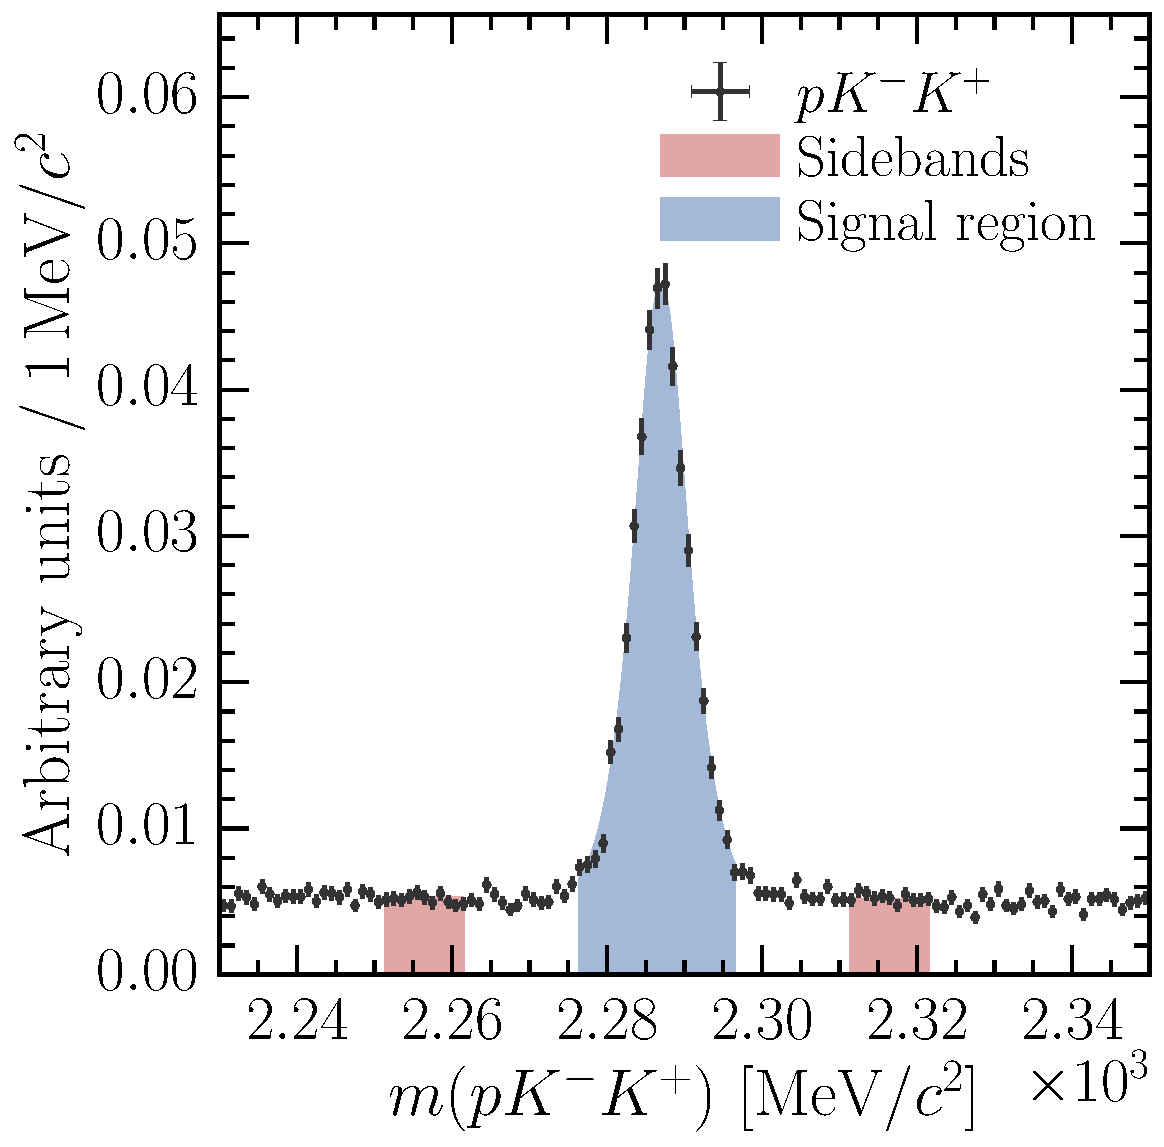
\includegraphics[width=\textwidth]{cpv/systematics/LcTopKK_2012_MagDown_Lb_DTF_Lc_M.pdf}
    \caption{\pKK}
    \label{fig:cpv:syst:mass_windows:pKK}
  \end{subfigure}
  \begin{subfigure}[b]{0.5\textwidth}
    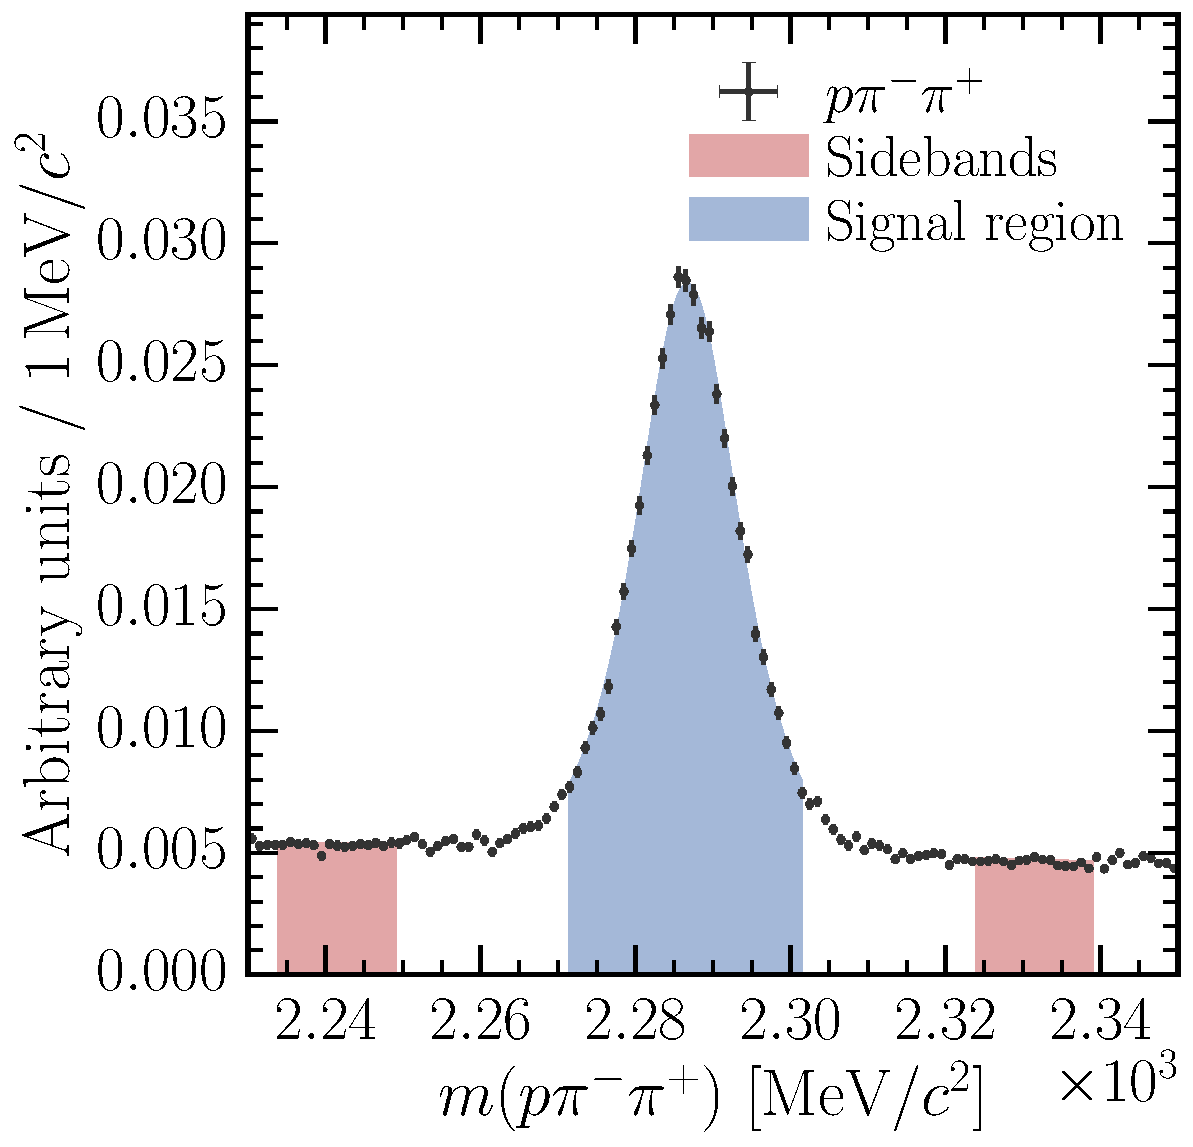
\includegraphics[width=\textwidth]{cpv/systematics/LcToppipi_2012_MagDown_Lb_DTF_Lc_M.pdf}
    \caption{\ppipi}
    \label{fig:cpv:syst:mass_windows:ppipi}
  \end{subfigure}
  \caption{%
    Definitions of the signal and sideband regions in the \PLambdac\ mass 
    spectrum for \pKK~(\subref*{fig:cpv:syst:mass_windows:pKK}) and 
    \ppipi~(\subref*{fig:cpv:syst:mass_windows:ppipi}).
    The 2012 magnet down data is overlaid for reference.
  }
  \label{fig:cpv:syst:mass_windows}
\end{figure}

\subsection{Results}
\label{chap:cpv:syst:fit:results}

For each data sub-sample, the \pKK\ and \ppipi\ samples are split by the charge 
of the \PLambdac\ and the sideband subtraction technique is used to measure the 
yields.
The yield asymmetry is then
\begin{equation}
  \ARaw(f) = \frac{%
    (N_{\text{S}}(\PLambdac) - N_{\text{SB}}(\PLambdac)) -
    (N_{\text{S}}(\APLambdac) - N_{\text{SB}}(\APLambdac))
  }{%
    (N_{\text{S}}(\PLambdac) - N_{\text{SB}}(\PLambdac)) +
    (N_{\text{S}}(\APLambdac) - N_{\text{SB}}(\APLambdac))
  },
  \label{eqn:cpv:syst:fit:araw_sb}
\end{equation}
where $N_{\text{S(SB)}}(\PLambdac)$ is the number of candidates in the signal 
(sideband) region in the \PLambdac\ sample, and $N_{\text{S(SB)}}(\APLambdac)$ 
is the same but in the \APLambdac\ sample.
The counts are assumed to be Poisson-distributed, and so the uncertainty 
$\unc{N}$ on each count is taken to be $\unc{N} = \sqrt{N}$.

The difference \dACP\ between \ARaw\ for \pKK\ and \ppipi\ is then computed 
using the values obtain with \cref{eqn:cpv:syst:fit:araw_sb}, and the 
difference is computed between those values and the nominal measurements given 
in \cref{tab:results:asymmetries}.
The uncertainty on \ARaw\ is found by propagating the uncertainties on the 
candidate counts using an \ac{MC} error propagation, and the values are assumed 
to be fully correlated with those from the nominal procedure.
The deviation from the nominal values is taken as a systematic uncertainty on 
\dACP\@.

\section{Residual background asymmetries}
\label{chap:cpv:syst:asym}

To do.

\section{Efficiency modelling}
\label{chap:cpv:syst:eff}

To do.
